% Pursuing Stacks (cotes 134-2 to 134-8): archive cote 134-6, site page 12 (PDF page 13), typescript page 331.
% typescript. Draft compared: ps5.tex:1938-2010.
% AI-transcribed by Claude Opus 5.5 (claude-opus-5-5, adaptive thinking, effort high), Message Batches API, batch ps3 (msgbatch_01XdFmuVVBAcgc7EFxdtCqsj), 2026-11-12; reviewed against both supplied scan halves; see CHECK_DECISIONS.tsv.
\scanpage{134-6/12}
\mspage{331}

functor
\[ (27) \qquad \mathrm{Add}(j\hand{{}^{\circ}}) : \mathrm{Add}(\hand{\Delta^{\circ}}) \hand{\longrightarrow} \mathrm{Add}(A^{\circ}) \ , \]
hence we get an $L.$ as the \xout{canonical} image of the canonical chain com-%
plex $L.^{\hand{\Delta}}$ we got in $\mathrm{Add}(\hand{\Delta}^{\circ})$.

6.7.

93. It is time to give the promised construction of Add(B), \xout{for any}
\xout{category B} the additive envelope of B, for any given category B.
The obvious idea is to enlarge the sets Hom(a,b), for a and b in B,
by taking linear com\over[typed]{i}{b}\over[typed]{b}{i}nations with coefficients in $\underline{Z}$ i.e. writing
\[ (1) \qquad \mathrm{Hom}_{\mathrm{Add}(B)}(a,b) = \underline{Z}^{(\mathrm{Hom}(a,b))} \ , \]
and composing these $\mathrm{Hom}_{\mathrm{Add}}$ in the obvious way. This is not quite
enough though, as we still have to add new objects, namely direct sums
of objects in B. The most convenient way for doing so seems by defining
an object of Add(B) to be defined by a finite set I (in the given
universe), namely the indexing set for taking the direct sum, and
a map
\[ I \hand{\longrightarrow} \mathrm{Ob}\, \over{B}{B} \ , \]
in other words the new objects are just \uline{families} of objects \xout{fa} \inserted{of B}
\[ (\over[typed]{a}{b}_i)_{i\hand{\in} I} \ , \]
\deleted{of B} indexed by finite sets. We'll however denote by
\[ (\over[typed]{1}{2}) \qquad \hand{\bigoplus_{i\in I}} b_i \]
the corresponding object of Add(B), as this will turn out to be the
direct sum indeed of the images of the $b_i$'s in Add(B) - but of cour-%
se we'll ignore the possible existence of direct sums in B \xout{when} itself,
when they exist, and not confuse (1) with a direct sum taken in B.
Writing Homadd i\over{n}{n}\over{s}{s}tead of $\mathrm{Hom}_{\mathrm{Add}(B)}$ for the sake of abbreviation,
the maps between objects (1) are defined \over[typed]{h}{b}\over[typed]{\unsure{u|v}}{y} matrices in the obvious \over{w}{w}\over{a}{a}\over{\unsure{y}}{y}
\[ (3) \margin{\begin{tikzpicture}[x=.35em,y=.65em,baseline=-.5ex]\draw (0,0)--(0,1);\draw[->,color=blue] (2.7,1)--(0,1);\draw[->,color=blue] (2.7,0)--(0,0);\end{tikzpicture}} \qquad \mathrm{Homadd}((a_i)_{i\hand{\in} I},(b_j)_{j\hand{\in} J}) = \hand{\{}(u_{ij})_{(i,j)\hand{\in} I\times J} \hand{\mid} u_{ij} \hand{\in} \]
% Hand-drawn continuation cue wraps the second formula row and points upward.
\[ 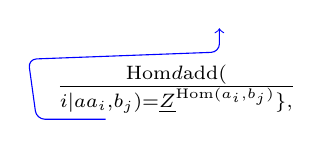
\begin{tikzpicture}[baseline=(continuation.base)]\node[inner sep=2pt] (continuation) {\ensuremath{\mathrm{Hom}\xout{d}\mathrm{add}(\over{\unsure{i|a}}{a}_i,b_j) = \underline{Z}^{\mathrm{Hom}(a_i,b_j)}\hand{\}} \hand{,}}};\draw[rounded corners=3pt,->,color=blue] ([xshift=2em]continuation.south west)--([xshift=-.5em]continuation.south west)--([xshift=-.8em]continuation.north west)--([xshift=-3em,yshift=.6ex]continuation.north east)--++(0,2ex);\end{tikzpicture} \]
while composition of maps is defined by the composition of matrices.
We thus get a new category Add(B) and a functor
\[ (4) \qquad B \hand{\longrightarrow} \mathrm{Add}(B) \ , \]

\margin{12}

% Visual collation: both supplied image halves inspected; see CHECK_DECISIONS_134_7_8.tsv.
